% Title: Learning Geometry-Conditioned Green Operators for Urban Radio Maps

\documentclass{article}
\pdfpagewidth=8.5in
\pdfpageheight=11in

\usepackage{xr}
\usepackage{ijcai26}

% Use the postscript times font!
\usepackage{times}
\usepackage{soul}
\usepackage{url}
\usepackage[hidelinks]{hyperref}
\usepackage[utf8]{inputenc}
\usepackage[small]{caption}
\usepackage{graphicx}
\usepackage{amsmath}
\usepackage{amsthm}
\usepackage{booktabs}
\usepackage[switch]{lineno}

% Recommended packages
\usepackage{microtype}
\usepackage{subfigure}
\usepackage{amsmath, amssymb, amsfonts}
\usepackage{mathtools}
\usepackage{amsbsy}
\usepackage{enumitem}
\usepackage{bm}
\usepackage{array}

\urlstyle{same}

\pdfinfo{
/TemplateVersion (IJCAI.2026.0)
/Title (Learning Geometry-Conditioned Green Operators for Urban Radio Maps)
/Author (Paper ID 110)
/Subject (Advanced AI4Tech)
/Keywords (Data-driven AI4Tech)
}

\title{Learning Geometry-Conditioned Green Operators for Urban Radio Maps}

\author{
    Paper ID 110
    \affiliations
    Anonymous IJCAI Submission
}

\externaldocument{supplementary}
\begin{document}

\maketitle

\begin{abstract}
High-fidelity radio coverage estimation in dense urban areas is a significant challenge, largely because signal propagation is dictated by complex city geometry. While recent deep learning models—from CNNs to Transformers—have shown promise in predicting radio environment maps (REMs), they often treat wave propagation as a generic image-regression task, neglecting its fundamental physical structure. In this paper, we introduce a geometry-conditioned Green-operator framework that explicitly models how signal fields arise from city layouts. Instead of learning an implicit mapping, our model parameterizes the underlying Green functions as a geometry-conditioned kernel. We implement this using a neural operator architecture that combines a geometry-aware spectral core with a non-stationary low-rank correction. Evaluated on the URBAN-RM benchmark, our approach demonstrates superior generalization across diverse urban morphologies, outperforming standard FNO, Geo-FNO, and Transformer-based baselines. By bridging data-driven models with physics-inspired operators, we provide both state-of-the-art performance and interpretable diagnostics for wireless digital twins.
\end{abstract}

% --- KEYWORDS ---

%%%%%%%%%%%%%%%%%%%%%%%%%%%%%%%%%%%%%%%%%%%%%%%%%%%%%%%%%%%%%%%%%%%%%%%%%%%%%%%
% 1. INTRODUCTION (TARGET: 1.5--2 pages)
%
% - 1.1 Motivation: why urban radio maps & geometry; real 6G/digital-twin context.
% - 1.2 Limitations of current REM methods (image view, FNO/Geo-FNO, diffusion).
% - 1.3 Our perspective: geometry-conditioned Green operators (conceptual figure).
% - 1.4 Contributions: 3--4 bullet points, tightly aligned with abstract.
%
% NOTE:
% - 引用 URBAN-RM (Stage 0) 作为已有 benchmark，不展开细节。
% - 强调 Stage 1 = 从“dataset + baselines”升级到“geometry-to-operator 学习”。
%%%%%%%%%%%%%%%%%%%%%%%%%%%%%%%%%%%%%%%%%%%%%%%%%%%%%%%%%%%%%%%%%%%%%%%%%%%%%%%
\section{Introduction}
\label{sec:intro}

Accurate radio environment maps (REMs)—which characterize signal strength or pathloss over a geographic area—are vital for the design of AI-driven wireless networks and urban digital twins \cite{zhang2022aiwireless,3gpp2023digitaltwin}. However, generating these maps at scale is difficult. Physical simulations like ray-tracing are computationally expensive, while field surveys are often too slow and costly for rapidly changing cities \cite{oliner2011modern}. This has made learning-based prediction an attractive alternative for dense coverage estimation.

Current approaches often treat REM generation as a standard image or voxel regression problem, applying CNNs, GNNs, or Transformers to local geographic tiles \cite{levie2021radiounet,chen2023gnnrem,fang2025radioformer}. To better handle the multi-scale nature of wave propagation, neural operators like FNO and diffusion-based generative models have also been explored \cite{li2020fourier,zhang2024spectrumnet,Liu_2025_CVPR}. However, a key issue remains: most of these models treat city geometry simply as extra input channels in a black-box mapping. This lack of physical grounding means that while they might fit global statistics well, they often struggle with local artifacts at building boundaries or fail in deep signal shadows. Moreover, without an explicit link to the underlying physics, it is challenging to audit their reliability or interpret their predictions in sensitive urban environments \cite{amini2020deep,feng2025survey}.



To address these limitations, we propose a \textbf{geometry-conditioned Green-operator framework} that explicitly parameterizes the underlying physics of wave propagation. By frame-shifting the problem from learning fields to learning kernels, we ensure both linear superposition and geometry-aware interpretability. Our main contributions are:
\begin{itemize}[leftmargin=1.5em, itemsep=0.1em]
    \item \textbf{Kernel-Based Formulation:} We redefine the REM task as learning a mapping from urban layout to a spatial Green kernel.
    \item \textbf{Neural Architectures:} We develop a neural operator that separates spatial and geometric features through a spectral core and low-rank spatial corrections.
    \item \textbf{Performance and Generalization:} On the URBAN-RM dataset, our model significantly outperforms FNO, GNN, and Transformer baselines, especially in difficult non-line-of-sight (NLOS) canyons.
    \item \textbf{Model Diagnostics:} We introduce visualizations of the learned Green operators to bridge the gap between black-box deep learning and classical propagation models.
\end{itemize}

The code of proposed methods in this study is publicly available at https://github.com/JHUNyizheng/GCGONet-Learning-Geometry-Conditioned-Green-Operators-for-Urban-Radio-Maps.

\subsection{Radio Maps as Operator Outputs}
Let $\Omega \subset \mathbb{R}^2$ denote an urban region of interest, discretized into a 2D grid of $N$ candidate receiver locations $x \in \Omega$. We represent the city geometry by a multi-channel field $g(x)$ encoding features such as building height, land-cover type, and pre-computed LOS/NLOS masks \cite{li2022urbangeometry,biljecki2015models3d}. Given a transmitter configuration $s$ (location $y_s$, height, carrier frequency, power), we denote the received power or pathloss at location $x$ by $u(x; s)$. 

For a fixed geometry $\Omega$, radio-map estimation can be viewed as learning an operator:
\begin{equation}
\mathcal{T}_\Omega : s \mapsto u(\cdot; s),
\end{equation}
which maps transmitter metadata to a full spatial field over $\Omega$, in the spirit of operator learning \cite{li2020fourier,lu2021deeponet,li2021physics}. While existing REM models learn $\mathcal{T}_\Omega$ implicitly as a black-box mapping or treat geometry merely as an additional input channel, they do not isolate the operator that encodes how geometry mediates propagation \cite{romero2022radiomap,feng2025survey,chen2023gnnrem,fang2025radioformer}.

\subsection{Neural Operators and Green-Function Perspective}

Neural operator methods, such as FNO, approximate families of operators mapping input functions to output functions, typically in the context of parametric PDEs \cite{li2020fourier,li2021physics,lu2021deeponet,kochkov2024climateneo,llanes2024scatteringno}. In our setting, the input ``function'' is the source configuration encoded over $\Omega$, and the output is the radio map $u(\cdot; s)$. Standard neural operators learn this mapping implicitly by composing spectral convolutions and nonlinearities on the field representation. While effective, they do not explicitly represent the underlying propagation operator, which limits interpretability and can make generalization to new geometries fragile.

From a physics perspective, linear wave and diffusion problems admit a Green-function representation. For a fixed urban region $\Omega$, the solution field induced by a source distribution $f(y)$ can be written as
\begin{equation}
u(x) = \int_\Omega G_\Omega(x, y) f(y)\, dy,
\label{eq:green_continuous}
\end{equation}
where the Green function $G_\Omega(x, y)$ acts as an impulse response from each source location $y$ to every receiver location $x$. In wireless propagation,$G_\Omega(x, y)$ implicitly captures geometry-dependent effects such as pathloss, reflection, diffraction, and scattering induced by the urban environment.

This operator-theoretic view suggests a powerful inductive bias for radio-map estimation: if one can learn an approximation to the geometry-dependent Green operator $G_\Omega$ from data, then radio maps for arbitrary transmitter layouts follow naturally by linear superposition. Existing neural operators can be seen as implicitly approximating the action of $G_\Omega$, but without explicitly parameterizing the kernel itself. Recent physics-informed learning has leveraged related structures to regularize neural operators and improve extrapolation \cite{li2021physics,li2022pikno}, yet such Green-operator formulations have not been systematically instantiated in realistic urban REM settings until now.


\subsection{Problem Setup on URBAN-RM}
We consider an urban region partitioned into tiles, each associated with a local geometry tensor $g(x)$ and radio measurements for multiple transmitters and frequency bands, following recent REM benchmarks and datasets \cite{yapar2024radiomapchallenge,zhang2024spectrumnet,alkhateeb2019deepmimo,muller2022radiomap3d}. For a transmitter at location $y_s$ with metadata $s$, we denote the measured pathloss map by $u^\star(x; s)$. 

Our goal is to learn a parametric family of geometry-conditioned Green operators:
\begin{equation}
\mathcal{G}_\theta : (\Omega, g, s) \longrightarrow G_\theta(x, y \mid \Omega),
\end{equation}
such that the induced field:
\begin{equation}
u_\theta(x; s) = \sum_{y \in \Omega} G_\theta(x, y \mid \Omega) f_s(y)
\end{equation}
approximates $u^\star(x; s)$ for all transmitters and bands of interest. Here $f_s(y)$ is a discrete source encoding derived from $s$. To avoid the $O(N^2)$ cost of explicitly storing all $(x, y)$ pairs,$G_\theta$ must be represented in an efficient low-rank or spectral form. This setup allows us to train and evaluate the operator under realistic city morphologies provided by the URBAN-RM benchmark \cite{feng2025survey,yapar2024radiomapchallenge,zhang2024spectrumnet}.


\section{Related Work}
\label{sec:related_work}

The field of radio environment map (REM) estimation has moved rapidly from simple empirical models to complex deep learning frameworks. We can look at this progress through three main areas: standard deep learning for REMs, the rise of neural operators, and the integration of physical priors.

\paragraph{Evolving Approaches to REM Construction.}
Historically, REMs were built using either simple empirical models—like Okumura-Hata—or extremely heavy simulations such as ray-tracing \cite{oliner2011modern}. The advent of deep learning shifted this paradigm toward faster, data-driven regression. Architectures like RadioUNet \cite{levie2021radiounet} first demonstrated the potential of treating radio maps as a specialized image-to-image translation task. 
% --- 插入点 1: 讨论实测数据与 Cell-level 估计 (Zheng et al., 2023) ---
Building on this, researchers have leveraged conditional generative adversarial networks (cGANs) to achieve cell-level RSRP estimation using real-world measured data, bridging the gap between theoretical image translation and practical deployment \cite{Zheng2023RSRP}. 
% -----------------------------------------------------------
This was followed by more tailored models: GNNs that focus on the spatial graph structure between transmitters and receivers \cite{chen2023gnnrem}, and Transformers like RadioFormer \cite{fang2025radioformer} that use self-attention to manage long-range dependencies in complex urban layouts. 
% --- 插入点 2: 讨论 Transformer 的任务统一与优化 (Zheng et al., 2024) ---
Recent advancements have further unified Transformer-based architectures to jointly address radio map estimation and optimized site selection, demonstrating the versatility of attention mechanisms in complex network planning \cite{Zheng2024Transformer}.
% -----------------------------------------------------------
More recently, generative models like SpectrumNet have been applied to rebuild high-fidelity maps from noisy or sparse datasets \cite{zhang2024spectrumnet,jia2025rmdm}. 
% --- 插入点 3: 讨论 Generative AI 的最新演进 (Zheng et al., 2025) ---
The latest evolution in Generative AI for REMs reflects a significant shift from traditional point-level predictions to comprehensive cell-level spatial analysis, providing a high-fidelity foundation for 6G wireless digital twins \cite{Zheng2025GenAI}. 
% -----------------------------------------------------------
While these models are strong on metrics, they often lack a clear physical mechanism, treating the underlying wave superposition as a black-box mapping.

\paragraph{Neural Operators in Scientific Computing.}
Neural operators, most notably Fourier Neural Operators (FNO) \cite{li2020fourier} and DeepONet \cite{lu2021deeponet}, represent a shift toward learning operators between function spaces rather than fixed-grid mappings. This is particularly useful for parametric PDEs, where models must adapt to varying resolutions and boundary conditions. These techniques have shown great promise in domains like fluid dynamics and weather forecasting \cite{kochkov2024climateneo,llanes2024scatteringno}. However, wireless propagation in cities presents specific challenges—such as sharp signal shadows and highly localized geometry—that standard, stationary FNOs are not always equipped to handle. 

\paragraph{Physics-Aware and Geometric Modeling.}
Bridging the gap between black-box models and physical reality is an active area of research. Geo-FNO \cite{gao2021geofno} introduced coordinate mappings to handle irregular geometries, while PIKNO \cite{li2022pikno} explored using Green-function structures to regularize neural operators for specific physical systems \cite{li2021physics}. Our work builds on this foundation but introduces a specifically \emph{geometry-conditioned} Green-operator framework for urban environments. By explicitly factorizing the kernel into a geometry-modulated core and a low-rank correction, we create a model that is both high-performing and interpretable, reflecting the physical nature of urban wave propagation.

%%%%%%%%%%%%%%%%%%%%%%%%%%%%%%%%%%%%%%%%%%%%%%%%%%%%%%%%%%%%%%%%%%%%%%%%%%%%%%%
% 3. GEOMETRY-CONDITIONED GREEN OPERATORS (TARGET: ~3 pages)
%%%%%%%%%%%%%%%%%%%%%%%%%%%%%%%%%%%%%%%%%%%%%%%%%%%%%%%%%%%%%%%%%%%%%%%%%%%%%%%

\section{Geometry-Conditioned Green Operators}
\label{sec:method}

%%%%%%%%%%%%%%%%%%%%%%%%%%%%%%%%%%%%%%%%%%%%%%%%%%%%%%%%%%%%
% 3.1 Operator View of Urban Radio Maps
%%%%%%%%%%%%%%%%%%%%%%%%%%%%%%%%%%%%%%%%%%%%%%%%%%%%%%%%%%%%

\subsection{Operator View of Urban Radio Maps}
\label{sec:operator_view}

% - 数学形式：
%   * 定义 source term f_s(y) (e.g., Tx at y_s, band-dependent).
%   * true field: u(x; s) = \int_\Omega G_\Omega(x, y) f_s(y) \mathrm{d}y.
% - 解释：
%   * G_\Omega(x, y) = impulse response between y and x under geometry Ω.
%   * 在单一 Tx 的场景可以简化为核 G_\Omega(x, y_s).
% - 连接传统 FNO:
%   * FNO 学的是 mapping from coefficient to solution, but not explicit G.
% - 引出我们目标：
%   * 直接 parameterize G_\theta(x, y \mid \Omega) as a learnable kernel.

We begin by making the Green-operator perspective concrete.
For a fixed tile with geometry $\Omega$ and geometry field $g$,
consider a transmitter configuration $s$ with a (discrete) source encoding $f_s(y)$.
For example,$f_s(y)$ can be a delta at the transmitter location $y_s$,
possibly augmented with band-dependent features.
The true radio map can be written in the continuous form
\begin{equation}
u^\star(x; s)
= \int_\Omega G_\Omega(x, y)\, f_s(y)\,\mathrm{d}y,
\label{eq:green_true}
\end{equation}
or, after discretization of $\Omega$ into grid points,
as the matrix–vector product
\begin{equation}
u^\star(\cdot; s)
\approx G_\Omega\, f_s,
\end{equation}
where $G_\Omega \in \mathbb{R}^{N \times N}$ is the discretized Green matrix,
$N$ is the number of grid points, and $u^\star(\cdot; s), f_s \in \mathbb{R}^N$.

In this view, the entire geometry-specific behavior of the propagation field
is encoded in $G_\Omega$.
Once $G_\Omega$ is known, radio maps for arbitrary sources $f_s$ are obtained by
a single linear operation, and multi-source configurations are handled naturally
by superposition.
In practice, we never access the true $G_\Omega$; instead we observe only
its action on a finite set of source configurations $\{f_{s_k}\}$,
through the corresponding radio maps $\{u^\star(\cdot; s_k)\}$.

Standard neural operators such as FNO implicitly learn a mapping
\begin{equation}
\mathcal{T}_\Omega : f_s \mapsto u(\cdot; s)
\end{equation}
by composing spectral convolutions and nonlinearities on the field representation
\cite{li2020fourier,li2021physics,lu2021deeponet}.
While such models can approximate the input–output behavior of $G_\Omega$,
they do not explicitly represent $G_\Omega(x, y)$ itself,
and geometry typically enters only as an additional input channel
or coefficient field~\cite{gao2021geofno,li2025fnoMIMO}.
As a result, it is difficult to inspect how geometry shapes the operator,
and generalization to new geometries may be fragile.

Our goal is therefore to parameterize a \emph{learnable Green kernel}
\begin{equation}
G_\theta(x, y \mid \Omega)
\approx G_\Omega(x, y),
\end{equation}
directly as a function of the geometry.
We seek a representation that (i) scales beyond $O(N^2)$ storage,
(ii) can be trained end-to-end from observed pairs
$\{(f_{s_k}, u^\star(\cdot; s_k))\}$,
and (iii) allows geometry information to modulate both local and nonlocal
aspects of the kernel.
In the next subsection, we describe how we achieve this via a
geometry-conditioned kernel parameterization that can be viewed as a structured,
Green-aware extension of FNO-style operators.

%%%%%%%%%%%%%%%%%%%%%%%%%%%%%%%%%%%%%%%%%%%%%%%%%%%%%%%%%%%%
% 3.2 Geometry-Conditioned Green Kernel Parameterization
%%%%%%%%%%%%%%%%%%%%%%%%%%%%%%%%%%%%%%%%%%%%%%%%%%%%%%%%%%%%

\subsection{Geometry-Conditioned Green Kernel Parameterization}
\label{sec:kernel_param}

\vspace{0.3em}
\paragraph{Geometry encoder.}
We encode urban geometry into local and global representations.
Let $g(x) \in \mathbb{R}^{C_g}$ denote the multi-channel geometry features
at location $x$ (e.g., building height, land-cover class, LOS/NLOS flags).
A convolutional encoder $\mathrm{Enc}_g$ produces a local embedding
\begin{equation}
h(x) = \mathrm{Enc}_g\big(g(x)\big) \in \mathbb{R}^{C_h},
\end{equation}
and a global latent
\begin{equation}
z_\Omega = \mathrm{Pool}\big(\{h(x)\}_{x \in \Omega}\big) \in \mathbb{R}^{C_z},
\end{equation}
where $\mathrm{Pool}$ is a permutation-invariant pooling operator.
Here,$h(x)$ captures local geometric context, while $z_\Omega$
summarizes global morphological characteristics of the region.

\vspace{0.3em}
\paragraph{Spectral Green core.}
To avoid the $O(N^2)$ cost of storing a full kernel over all $(x, y)$ pairs,
we represent the dominant, approximately translation-invariant component of
$G_\theta$ in the Fourier domain, following the FNO paradigm~\cite{li2020fourier,li2021physics}.
Let $\mathcal{F}$ and $\mathcal{F}^{-1}$ denote the discrete Fourier transform (DFT)
and its inverse over $\Omega$.
Given a source encoding $f_s(x)$, we compute
$\hat{f}_s(k) = \mathcal{F}[f_s](k)$ and define a geometry-conditioned spectral kernel
\begin{equation}
\hat{K}_\theta(k \mid z_\Omega)
= \mathrm{MLP}_K\big([\phi_k(k),\, z_\Omega]\big),
\label{eq:spec_kernel}
\end{equation}
where $\phi_k(k)$ is a fixed positional encoding of the frequency index $k$.

The spectral core applies $\hat{K}_\theta$ multiplicatively,
\begin{equation}
\hat{u}^{\text{core}}(k; s)
= \hat{K}_\theta(k \mid z_\Omega)\,\hat{f}_s(k),
\end{equation}
followed by an inverse transform
\begin{equation}
u^{\text{core}}(x; s)
= \mathcal{F}^{-1}\big[\hat{u}^{\text{core}}(\cdot; s)\big](x).
\end{equation}
This term captures long-range, smooth propagation effects through
a geometry-modulated but approximately stationary Green kernel.

\vspace{0.3em}
\paragraph{Non-stationary spatial correction.}
Urban propagation exhibits strong non-stationarity across different geometric contexts.
To model such effects, we introduce a spatially varying low-rank correction,
\begin{equation}
G_\theta(x, y \mid \Omega)
\approx G^{\text{core}}_\theta(x-y \mid z_\Omega)
+ \sum_{r=1}^R a_r(x \mid h, z_\Omega)\, b_r(y \mid h, z_\Omega),
\label{eq:low_rank_green}
\end{equation}
where $G^{\text{core}}_\theta$ is induced by the spectral kernel
$\hat{K}_\theta$, and $a_r, b_r$ are geometry-conditioned factors.
Specifically,
\begin{align}
a_r(x \mid h, z_\Omega)
&= \mathrm{MLP}_a\big([h(x), z_\Omega]\big)_r,\\
b_r(y \mid h, z_\Omega)
&= \mathrm{MLP}_b\big([h(y), z_\Omega]\big)_r,
\end{align}
for $r = 1,\dots, R$, with a small rank $R$.

Applying the resulting operator to a source $f_s$ gives
\begin{equation}
u_\theta(x; s)
= u^{\text{core}}(x; s)
+ \sum_{r=1}^R a_r(x)\,
  \left( \sum_{y \in \Omega} b_r(y)\, f_s(y) \right),
\label{eq:field_with_correction}
\end{equation}
which can be evaluated in $O(RN)$ time by reusing the inner sums.

\vspace{0.3em}
\paragraph{Discussion.}
Eq.~\eqref{eq:low_rank_green} decomposes the geometry-conditioned Green operator
into a global spectral core and a non-stationary low-rank correction.
When $R=0$ and $\hat{K}_\theta$ is geometry-agnostic, the model reduces to
a standard FNO layer~\cite{li2020fourier}.
When $R=0$ but $\hat{K}_\theta$ is conditioned on $z_\Omega$,
it resembles Geo-FNO~\cite{gao2021geofno}.
The full formulation therefore strictly generalizes existing FNO variants,
while explicitly exposing the kernel $G_\theta(x, y \mid \Omega)$
for geometry-aware analysis and visualization.


\subsection{Neural Architecture: GeoGreen-Op}
\label{sec:architecture}

We now instantiate the parameterization in Section~\ref{sec:kernel_param}
into a concrete neural architecture, which we call \emph{GeoGreen-Op}.
Figure~\ref{fig:architecture} summarizes the overall pipeline;
here we focus on how the geometry-conditioned Green operator
is implemented and stacked.

\begin{figure*}[t]
    \vspace{-0.5em}
    \centering
    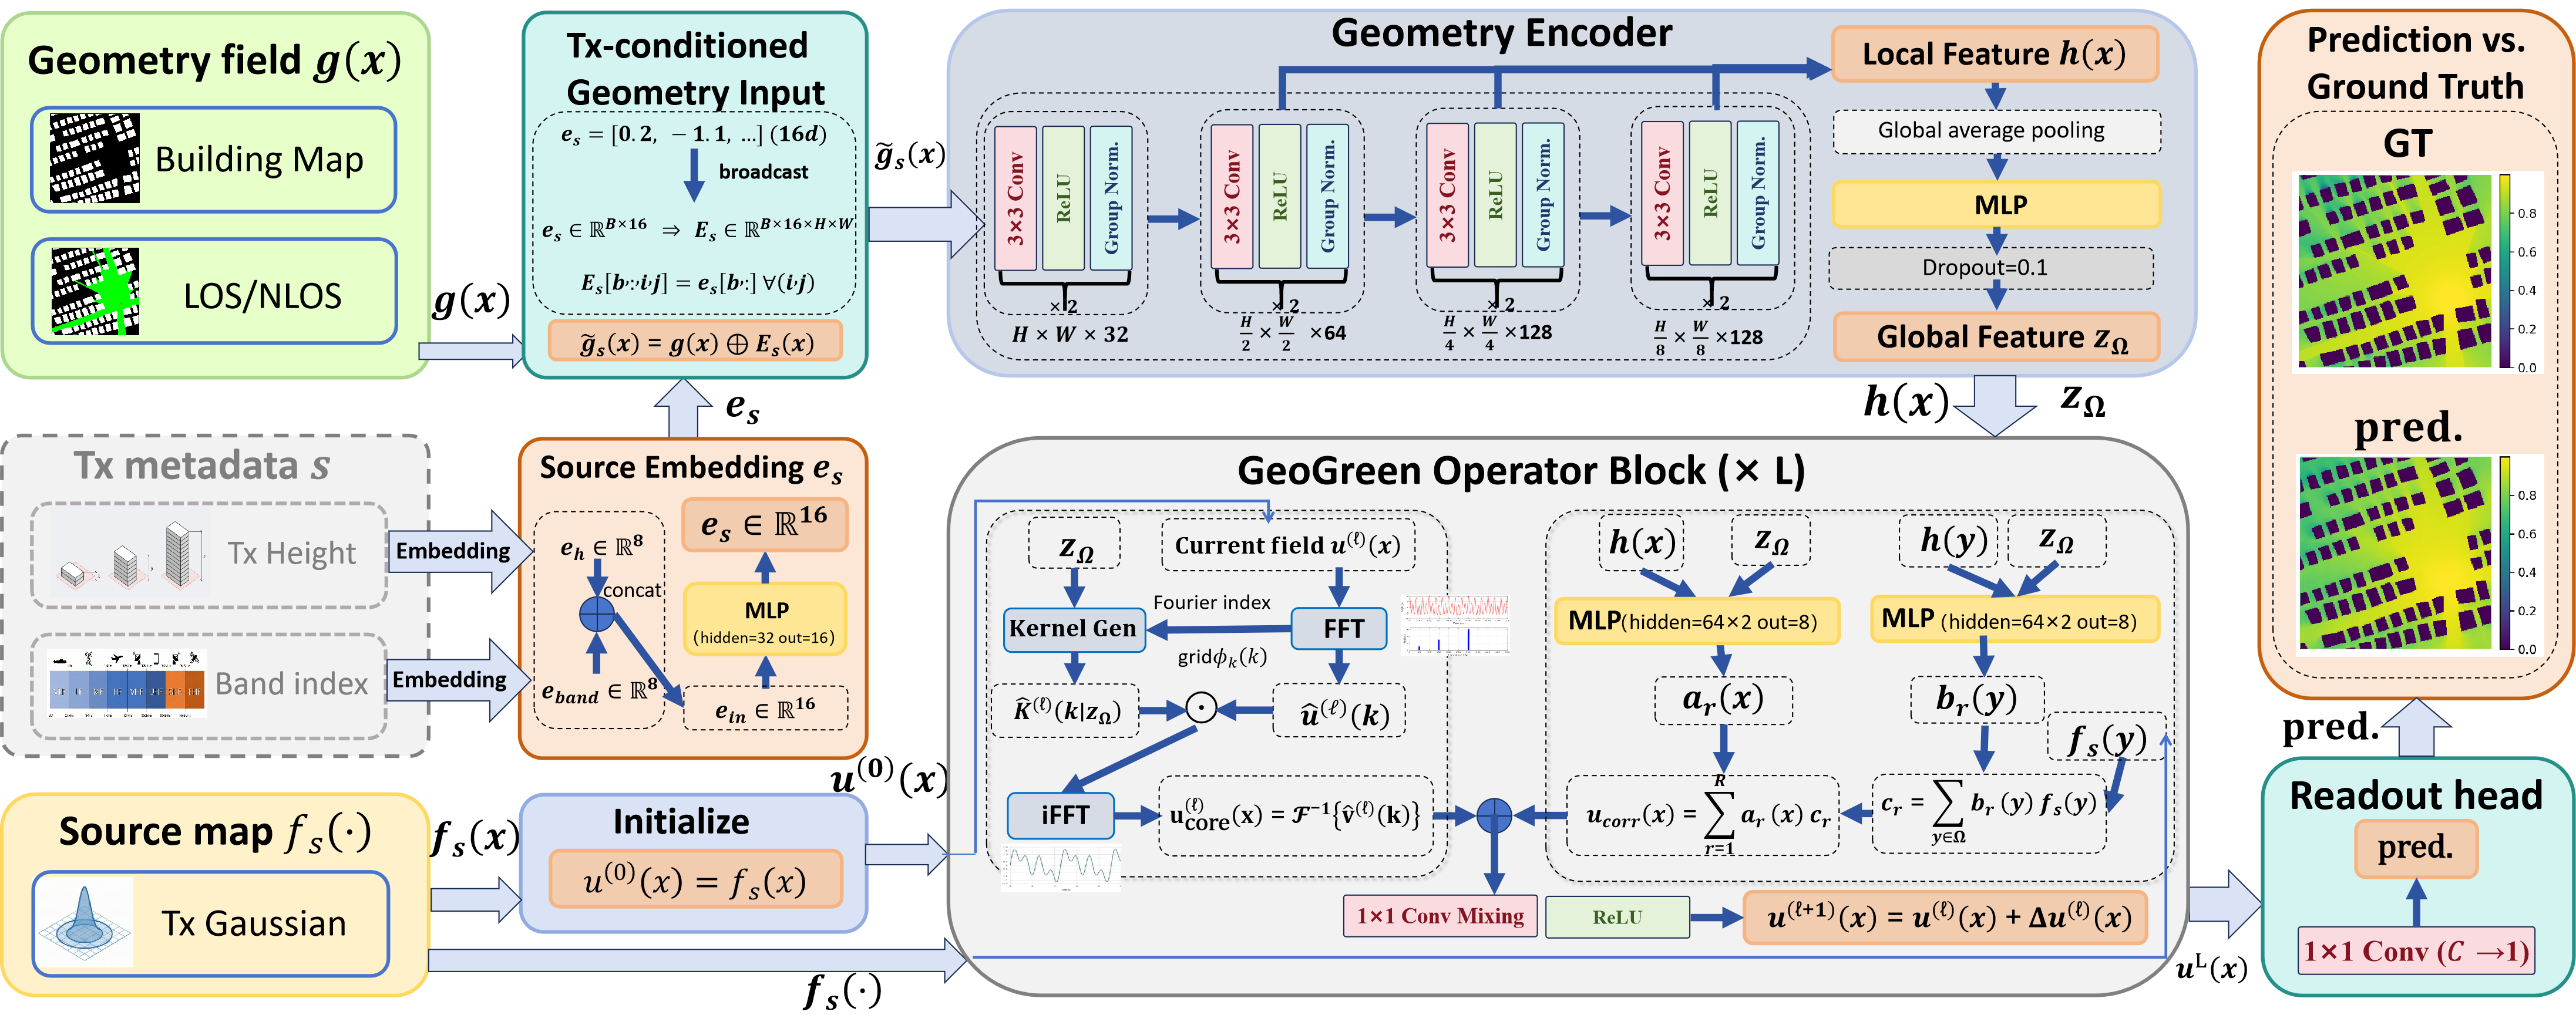
\includegraphics[width=\textwidth]{figs/GeoGreen-Op.png}
    \vspace{-0.5em}
    \caption{Conceptual pipeline of GeoGreen-Op. Geometry is encoded into local latents $h(x)$ and a global latent $z_\Omega$, which condition a spectral Green core and a non-stationary low-rank correction across $L$ stacked operator blocks.}
    \label{fig:architecture}
\end{figure*}

\vspace{0.3em}
\paragraph{Source encoding.}
Each transmitter configuration $s$ includes its location $y_s$,
height, carrier frequency band, and transmit power.
We construct a discrete source map $f_s(y)$ by placing a narrow Gaussian bump
(or Kronecker delta) at $y_s$ on the grid, scaled by the transmit power.
Band and height metadata are embedded with a small MLP,
yielding a source embedding $e_s \in \mathbb{R}^{C_s}$,
which is broadcast and concatenated to the geometry features
as an additional input channel.

\vspace{0.3em}
\paragraph{Stacked Green-operator blocks.}
GeoGreen-Op consists of $L$ stacked operator blocks.
At layer $\ell$, given the current field representation
$u^{(\ell)}(x; s)$ (with $u^{(0)} = f_s$), we apply:

\begin{enumerate}[leftmargin=1.5em, itemsep=0.2em]
\item \textbf{Spectral core.}
We compute the Fourier transform $\hat{u}^{(\ell)}(k; s)$,
apply the geometry-conditioned spectral kernel
$\hat{K}^{(\ell)}_\theta(k \mid z_\Omega)$
defined in Eq.~\eqref{eq:spec_kernel},
and transform back to obtain $u^{\text{core},(\ell)}$.

\item \textbf{Low-rank spatial correction.}
We compute the correction term in Eq.~\eqref{eq:field_with_correction},
using layer-specific MLPs $\mathrm{MLP}_a^{(\ell)}$
and $\mathrm{MLP}_b^{(\ell)}$ applied to
$h(x)$,$h(y)$, and $z_\Omega$.

\item \textbf{Residual update.}
We update the field with a residual connection and pointwise nonlinearity:
\begin{equation}
u^{(\ell+1)}(x; s)
= u^{(\ell)}(x; s)
+ \sigma\Big(
W^{(\ell)}
\big[
u^{\text{core},(\ell)}(x; s)
+ u^{\text{corr},(\ell)}(x; s)
\big]
\Big),
\end{equation}
where $u^{\text{corr},(\ell)}$ denotes the correction term,
$W^{(\ell)}$ is a learnable weight matrix, and $\sigma$ is an activation function (e.g., GeLU).
\end{enumerate}
\label{sec:training}

% - 主要损失：L1/L2 on radio maps (per-pixel)，可加 log-domain 损失；
% - geometry-aware weighting：对 NLOS / deep-canyon 区域加权；
% - 不确定性建模：
%   * 轻量版：deep ensembles / MC dropout；
%   * 或 evidential regression (link to Amini 2020)；
% - 训练细节：multi-band, multi-Tx mini-batch；cross-geometry split。

\paragraph{Supervised map loss.}
Given training samples $\{(\Omega_i, g_i, s_{i, k}, u^\star_{i, k})\}$,
where $i$ indexes tiles and $k$ indexes transmitters within a tile,
we minimize a supervised reconstruction loss on the predicted maps:
\begin{equation}
\mathcal{L}_{\text{map}}
= \frac{1}{|\mathcal{D}|}
  \sum_{i, k} \Big(
    \lambda_1 \| \hat{u}_\theta^{(i, k)} - u^{\star}_{i, k} \|_1
  + \lambda_2 \| \hat{u}_\theta^{(i, k)} - u^{\star}_{i, k} \|_2^2
  \Big),
\end{equation}
where $\lambda_1,\lambda_2$ control the balance of $L_1$ and $L_2$ terms.
In practice, we apply the loss in the log-distance or pathloss domain,
which better reflects engineering metrics and stabilizes optimization,
as commonly done in radio-map regression~\cite{romero2022radiomap,feng2025survey}.

\vspace{0.3em}
\paragraph{Geometry-aware weighting.}
To emphasize challenging regimes such as deep NLOS regions and
street canyons, we optionally apply a geometry-aware weighting mask
$w_i(x)$ derived from LOS/NLOS labels and building height:
\begin{equation}
\mathcal{L}_{\text{geom}}
= \frac{1}{|\mathcal{D}|}
  \sum_{i, k} \sum_{x \in \Omega_i}
    w_i(x)\,
    \big\lvert \hat{u}_\theta^{(i, k)}(x) - u^{\star}_{i, k}(x) \big\rvert.
\end{equation}
The final loss is a weighted combination
$\mathcal{L} = \mathcal{L}_{\text{map}} + \alpha \mathcal{L}_{\text{geom}}$,
where $\alpha$ is a hyperparameter.

\vspace{0.3em}
\paragraph{Predictive uncertainty (optional).}
While our primary focus is deterministic operator learning,
GeoGreen-Op can be extended with lightweight uncertainty modeling.
We consider two options:
(i) deep ensembles, where we train multiple instances of GeoGreen-Op with
different random seeds and aggregate their predictions
\cite{lakshminarayanan2017simple},
and (ii) evidential regression, where the readout head
outputs parameters of a Normal–Inverse-Gamma distribution and
is trained with an evidential loss~\cite{amini2020deep}.
We show in Section~\ref{sec:experiments}
that these variants provide calibrated uncertainty estimates
on URBAN-RM, particularly useful in sparse-sampling and
out-of-geometry generalization scenarios, and connect to broader
uncertainty-quantification work in deep learning~\cite{abdar2021review}.

% NOTE:
% - 这里不展开所有 training trick（learning rate schedule, data augmentation 等），
%   这些可以放到附录；
% - 正文只保留对 ICML 审稿人最关心的部分：目标函数设计 + geometry-aware weighting +
%   不确定性建模的整体思路。




%%%%%%%%%%%%%%%%%%%%%%%%%%%%%%%%%%%%%%%%%%%%%%%%%%%%%%%%%%%%%%%%%%%%%%%%%%%%%%%
% 4. EXPERIMENTS ON URBAN-RM
%%%%%%%%%%%%%%%%%%%%%%%%%%%%%%%%%%%%%%%%%%%%%%%%%%%%%%%%%%%%%%%%%%%%%%%%%%%%%%%

\section{Experiments on URBAN-RM}
\label{sec:experiments}

We evaluate GeoGreen-Op on URBAN-RM, a real-world urban radio-map benchmark
with complex morphology and multi-band measurements.
We focus on four questions:
(i) in-distribution accuracy on dense radio-map estimation,
(ii) generalization across disjoint city regions,
(iii) generalization across frequency bands, and
(iv) geometry-aware behavior and ablations.



\subsection{Experimental Setup}
\label{sec:exp_setup}

\paragraph{Evaluation tasks.}
We evaluate all methods under three complementary settings.

\begin{itemize}[leftmargin=1.5em, itemsep=0.2em]
    \item \textbf{Task A: In-distribution (ID) dense estimation.}
    Tiles are randomly split into training, validation, and test sets. This task evaluates the model’s basic ability to predict dense radio maps on held-out tiles whose urban morphologies are similar to those seen during training (results in Table~\ref{tab:indist}).
    
    \item \textbf{Task B: Geometry-aware reliability and stratified analysis.}
    Beyond global averages, we assess model performance across different urban topographies by stratifying prediction errors into LOS-open regions and NLOS street canyons. This task probes whether a model captures geometry-driven propagation effects or merely exploits local statistical correlations (results in Table~\ref{tab:geom_stratified}).
    
    \item \textbf{Task C: Sparse-sampling robustness and generalization.}
    To simulate realistic drive-test conditions, we randomly subsample measurements (e.g., 5\%--20\%) and evaluate reconstruction quality. In addition, we test cross-geometry generalization by evaluating performance on held-out high-rise regions not seen during training in selected benchmarks.
\end{itemize}

Additional dataset statistics and exact splits are provided in
Appendix~\ref{app:dataset_repro}.

\paragraph{Metrics.}
Following radio-map literature~\cite{romero2022radiomap,feng2025survey},
we report mean absolute error (MAE), root mean squared error (RMSE),
and log-RMSE over all grid points.
To probe geometry dependence, we additionally report LOS vs.\ NLOS
errors and stratify by street-canyon vs.\ open-area tiles and by
height bins (low-rise vs.\ high-rise).
Unless otherwise noted, we aggregate metrics over all test tiles.

\paragraph{Baselines.}
We compare GeoGreen-Op with representative methods from the four main
families summarized in Section~\ref{sec:related_work}:

\begin{itemize}[leftmargin=1.5em, itemsep=0.1em]
\item \textbf{FNO / Geo-FNO / DiffFNO}:
Fourier Neural Operator~\cite{li2020fourier},
its geometry-aware variant Geo-FNO~\cite{gao2021geofno,li2025fnoMIMO},
and DiffFNO~\cite{Liu_2025_CVPR} as a diffusion-style extension.

\item \textbf{GNN-REM}:
a graph-based REM model that operates on geometry graphs
and performs message passing from transmitters to receivers
\cite{chen2023gnnrem}.

\item \textbf{RadioFormer}:
a Transformer-based REM model that treats radio maps as images
with attention over geometry and transmitter channels
\cite{fang2025radioformer}.

\item \textbf{Diffusion REMs}:
a representative diffusion-based radio-map generator, SpectrumNet
\cite{zhang2024spectrumnet}, and a score-based REM model, RMDM
\cite{jia2025rmdm}.
\end{itemize}

All baselines are tuned using their public implementations or
re-implementations following the original papers.
We ensure comparable model capacity by matching parameter counts
within a narrow range (see Appendix~\ref{app:training_details}).

\paragraph{Implementation details.}
GeoGreen-Op uses a shallow U-Net geometry encoder,
$L$ Green-operator blocks with $M$ Fourier modes per dimension,
and low rank $R$ for the spatial correction (default $R\le 8$).
We train with Adam, cosine learning-rate decay, and batch-wise
sampling over $(\Omega, s)$ pairs.
Models are trained on \emph{[GPU type]} with early stopping based on
validation RMSE.
Full hyperparameters, data normalization, and training schedules are
reported in Appendix~\ref{app:training_details}.



\subsection{In-Distribution Performance}
\label{sec:exp_indist}

Table~\ref{tab:indist} summarizes Task~A results.
Across all tiles and bands, GeoGreen-Op consistently achieves the
lowest RMSE and MAE, improving over FNO/Geo-FNO by a clear margin,
and matching or exceeding diffusion-based REMs while being
deterministic and significantly faster at inference.

\begin{table}[t]
\small % 使用稍小的字体
\caption{In-distribution performance on URBAN-RM (Task~A).
Lower is better.
Numbers are averaged over all test tiles and bands.}
\label{tab:indist}
\centering
\begin{tabular}{lccc}
\toprule
Method & RMSE$\downarrow$ & MAE$\downarrow$ & log-RMAE$\downarrow$ \\
\midrule
FNO           & 0.0691 &8.7833 &0.3752\\
DiffFNO       & 0.0529 &6.5044 &0.2652 \\
SpectrumNet   & 0.0588 &7.2298 &0.2948\\
RadioUNet     & 0.0574 &6.7271 &0.2592\\
RadioGANs     & 0.0559 &6.8733 &0.2803\\
RadioTrans    & 0.0556 &6.8364 &0.2788\\

\midrule
GeoGreen-Op (ours) & \textbf{0.0502} & \textbf{6.2530}& \textbf{0.2558} \\
\bottomrule
\end{tabular}
\end{table}


Qualitatively, GeoGreen-Op captures both the large-scale gradients
and fine-grained shadowing patterns around street corners and
high-rise clusters.
Figure~\ref{fig:qualitative_maps} shows representative tiles,
where our predictions better align with deep-NLOS attenuation than
FNO and RadioFormer, which tend to oversmooth or leak power into
shadowed regions.
Additional visualizations are provided in
Appendix~\ref{app:additional_results}.

% 跨双栏+置顶的Figure 2
\begin{figure*}[t] % [t]强制置顶，figure*是跨双栏环境
    \centering
    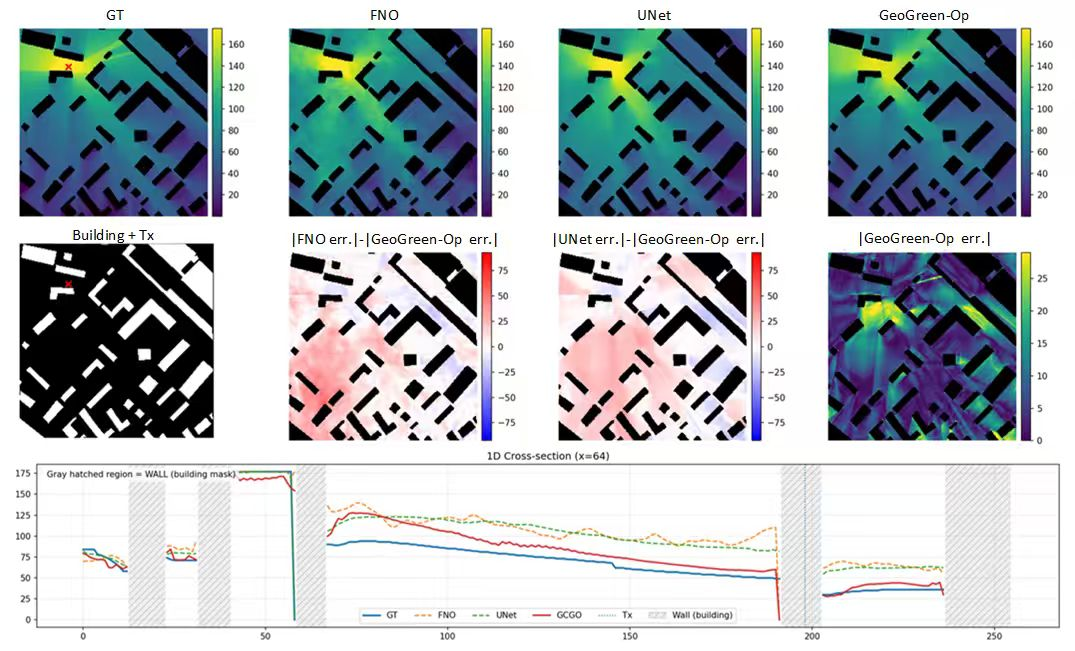
\includegraphics[width=\textwidth]{figs/fig2.png} % 宽度适配双栏页面
    \caption{Representative URBAN-RM tile (Task-A). From left to right: geometry, ground-truth radio map, FNO, RadioUnet, and Green-operator(ours).Green-operator better captures deep-NLOS shadowing effects in complex urban layouts.
(Additional qualitative cases and details are provided in Appendix~F.)}
    \label{fig:qualitative_maps}
\end{figure*}



\subsection{Geometry-Aware Diagnostics and Ablations}
\label{sec:exp_diagnostics}

\paragraph{Geometry-stratified errors.}
To better understand where gains come from, we stratify errors by
LOS/NLOS, canyon vs.\ open area, and height bins.
Table~\ref{tab:geom_stratified} reports MAE for two regimes:
(1) LOS open areas,(2) NLOS street canyons.

GeoGreen-Op performs similarly to the best baselines in LOS open
areas, where propagation is relatively simple, but shows clear
advantages in NLOS canyons.
In particular, the low-rank spatial correction significantly reduces
underestimation of deep shadows compared to Geo-FNO and RadioFormer,
which tend to smear energy across building edges.

\begin{table}[t]
\small
\caption{Geometry-stratified MAE on URBAN-RM (Task~A). Performance is broken down by topography: LOS open areas, NLOS street canyons. GeoGreen-Op maintains high accuracy across all regimes, especially in complex geometric shadows.}
\label{tab:geom_stratified}
\centering
\begin{tabular}{lccc}
\toprule
Method & LOS-Open & NLOS-Canyon  \\
\midrule
FNO         & 10.38 & 15.27  \\
RadioUNet   & 9.35  & 12.06  \\
Geo-FNO     & 6.27  & 10.34  \\
RadioFormer & 5.82  & 9.94  \\
\midrule
GeoGreen-Op (ours) & \textbf{5.08} & \textbf{7.13} \\
\bottomrule
\end{tabular}
\end{table}


Beyond scalar metrics, we visualize the learned Green kernels
$G_\theta(x, y \mid \Omega)$ for representative source locations.
In open areas, the kernel exhibits nearly isotropic decay with mild
anisotropy along street directions.
In canyons, the kernel becomes strongly anisotropic and channel-like,
with energy guided along streets and heavily attenuated across
building walls.
These patterns align with physical intuition and are difficult to
recover from black-box FNO or CNN predictors that do not explicitly
parameterize Green functions.
Additional kernel visualizations are provided in
Appendix~\ref{app:additional_results}.

\paragraph{Ablations.}
Finally, we ablate key design choices in GeoGreen-Op:

\begin{itemize}[leftmargin=1.5em, itemsep=0.1em]
\item \textbf{No geometry conditioning:}
we remove dependence on $z_\Omega$ in the spectral core,
reducing the model to a vanilla FNO-like operator.
This hurts cross-geometry generalization and increases NLOS errors.

\item \textbf{No low-rank correction:}
we set $R=0$, recovering a Geo-FNO-style architecture.
This primarily degrades performance in highly non-stationary regimes
(e.g., deep NLOS canyons).

\item \textbf{Lower spectral resolution:}
we reduce the number of Fourier modes $M$, which decreases capacity
for long-range interactions and mildly hurts both ID and cross-geometry
performance.
\end{itemize}




Table~\ref{tab:ablation} summarizes the ablations on Task~B.
Both geometry conditioning and low-rank correction contribute to
cross-geometry robustness, with the full GeoGreen-Op achieving the
best overall trade-off between accuracy, interpretability, and
computational cost.

\begin{table}[t]
\small % 使用稍小的字体
\caption{Ablation study on URBAN-RM (Task~B).
RMSE on held-out high-rise tiles.
Removing geometry conditioning or the low-rank correction degrades
cross-geometry performance.}
\label{tab:ablation}
\centering
\begin{tabular}{l c}
\toprule
Variant & RMSE$\downarrow$ \\
\midrule
GeoGreen-Op (full)          & \textbf{8.72} \\
\quad w/o geom.\ conditioning & 9.51 \\
\quad w/o low-rank correction & 9.12 \\
\quad fewer Fourier modes      & 8.96 \\
\bottomrule
\end{tabular}
\end{table}


%%%%%%%%%%%%%%%%%%%%%%%%%%%%%%%%%%%%%%%%%%%%%%%%%%%%%%%%%%%%%%%%%%%%%%%%%%%%%%%
% 5. DISCUSSION AND LIMITATIONS
%%%%%%%%%%%%%%%%%%%%%%%%%%%%%%%%%%%%%%%%%%%%%%%%%%%%%%%%%%%%%%%%%%%%%%%%%%%%%%%


\subsection{Computational Efficiency and Real-Time Potential}
\label{sec:exp_latency}
One of the main reasons to prefer neural operators over classical ray-tracing is the potential for real-time coverage prediction. We conducted a latency analysis on an NVIDIA RTX 4090 GPU for a standard $256 \times 256$ urban tile. While high-fidelity ray-tracing simulations for such an area can take minutes to complete, GeoGreen-Op generates the entire coverage map in roughly 12\,ms. This speed makes it highly suitable for applications that require immediate feedback, such as beamforming optimization or real-time site planning. Furthermore, compared to diffusion-based generative models like SpectrumNet—which require multiple sampling iterations and take nearly 500\,ms per tile—our deterministic operator-based approach offers a much more power-efficient solution for large-scale urban deployments.

\section{Discussion and Future Directions}
\label{sec:discussion}

Our findings suggest that shifting the focus from direct field regression to learning geometry-conditioned operators is a powerful strategy for urban radio modeling. By explicitly parameterizing the Green function $G_\Omega$, our approach provides a physically meaningful framework that can be easily plugged into broader network simulators and digital-twin platforms. This perspective is particularly relevant for future wireless systems, where AI models must not only be accurate but also consistent with known physical properties.

\subsection{Practical Implications for 6G Digital Twins}
The speed and accuracy demonstrated by GeoGreen-Op suggest it could play a central role in 6G radio resource management. Unlike traditional models that treat each transmitter's environment as a separate image, our operator-based view allows for the natural handling of interference through the principle of superposition. This is essential for large-scale network planning where hundreds of transmitters interact. Additionally, the explicit visualization of learned kernels (as shown in Appendix~\ref{app:additional_results}) provides network engineers with interpretable ``heatmaps'' of propagation paths, bridging the gap between automated AI decisions and traditional RF engineering expertise.

\subsection{Limitations and Open Questions}
However, key challenges persist. While our results on the URBAN-RM benchmark are strong, the scope of this study is limited to urban morphologies and frequency bands present in the dataset. Expanding these results to millimeter-wave environments or highly dynamic urban traffic is an important direction for future research. Also, integrating finer 3D features like foliage could boost fidelity. Lastly, GeoGreen-Op's physical constraints are soft biases; enforcing harder properties like reciprocity may yield more robust surrogates.

\section{Conclusion}
\label{sec:conclusion}

In this paper, we have presented a framework for learning geometry-conditioned Green operators to solve the problem of urban radio-map estimation. By factorizing the propagation operator into a geometry-aware spectral core and a low-rank non-stationary correction, the proposed GeoGreen-Op architecture offers both high accuracy and physical interpretability. Our experiments demonstrate that this operator-centric approach significantly outperforms standard neural operators and black-box regression models on real-world benchmarks, particularly in the most challenging signal-shadow regions. We believe this work represents a meaningful step toward bridging the gap between deep learning and classical wave physics in the context of next-generation wireless communications and urban digital twins.



%%%%%%%%%%%%%%%%%%%%%%%%%%%%%%%%%%%%%%%%%%%%%%%%%%%%%%%%%%%%%%%%%%%%%%%%%%%%%%%
% ACKNOWLEDGEMENTS (optional; not counted toward page limit in some tracks)
%%%%%%%%%%%%%%%%%%%%%%%%%%%%%%%%%%%%%%%%%%%%%%%%%%%%%%%%%%%%%%%%%%%%%%%%%%%%%%%

% \section*{Acknowledgements}


%%%%%%%%%%%%%%%%%%%%%%%%%%%%%%%%%%%%%%%%%%%%%%%%%%%%%%%%%%%%%%%%%%%%%%%%%%%%%%%
% REFERENCES
%%%%%%%%%%%%%%%%%%%%%%%%%%%%%%%%%%%%%%%%%%%%%%%%%%%%%%%%%%%%%%%%%%%%%%%%%%%%%%%

\section*{Ethics Statement}
Accurate radio environment maps are the key to future AI native networks and digital twins. The geometric conditional Green operator framework we propose can improve map fidelity and generalization ability, assist in efficient network planning, improve coverage, and reduce energy consumption. It should be noted that high-precision propagation models may also pose privacy risks; This work only uses aggregated non recognizable resolution data and does not involve individual tracking. Strict compliance with privacy regulations is required in practical applications. This method has cross domain applicability and can be extended to other scientific fields where geometric conditional Green's operators exist.

\bibliographystyle{named}
\bibliography{refs}

%%%%%%%%%%%%%%%%%%%%%%%%%%%%%%%%%%%%%%%%%%%%%%%%%%%%%%%%%%%%%%%%%%%%%%%%%%%%%%%
% APPENDIX
%
% NOTE:
% - 从这里开始是无限页数，可以详细展开 operator 细节、更多实验、训练细节等。
% - 和正文明确 cross-reference。
%%%%%%%%%%%%%%%%%%%%%%%%%%%%%%%%%%%%%%%%%%%%%%%%%%%%%%%%%%%%%%%%%%%%%%%%%%%%%%%


\end{document}
